\let\negmedspace\undefined
\let\negthickspace\undefined
\documentclass[journal,12pt,onecolumn]{IEEEtran}
\usepackage{cite}
\usepackage{amsmath,amssymb,amsfonts,amsthm}
\usepackage{algorithmic}
\usepackage{graphicx}
\graphicspath{{./figs/}}
\usepackage{textcomp}
\usepackage{xcolor}
\usepackage{txfonts}
\usepackage{listings}
\usepackage{enumitem}
\usepackage{mathtools}
\usepackage{gensymb}
\usepackage{comment}
\usepackage{mhchem}
\usepackage{caption}
\usepackage[breaklinks=true]{hyperref}
\usepackage{tkz-euclide} 
\usepackage{listings}
\usepackage{gvv}                                        
%\def\inputGnumericTable{}                                   
\usepackage[utf8]{inputenc}     
\usepackage{xparse}
\usepackage{color}                                            
\usepackage{array}                                            
\usepackage{longtable}                                       
\usepackage{calc}                                             
\usepackage{multirow}
\usepackage{multicol}
\usepackage{hhline}                                           
\usepackage{ifthen}                                           
\usepackage{lscape}
\usepackage{tabularx}
\usepackage{array}
\usepackage{float}
\newtheorem{theorem}{Theorem}[section]
\newtheorem{problem}{Problem}
\newtheorem{proposition}{Proposition}[section]
\newtheorem{lemma}{Lemma}[section]
\newtheorem{corollary}[theorem]{Corollary}
\newtheorem{example}{Example}[section]
\newtheorem{definition}[problem]{Definition}
\newcommand{\BEQA}{\begin{eqnarray}}
\newcommand{\EEQA}{\end{eqnarray}}
\newcommand{\define}{\stackrel{\triangle}{=}}
\theoremstyle{remark}
\newtheorem{rem}{Remark}

\usepackage{enumitem}
\setlist[enumerate,1]{label=\arabic*.}
\setlist[enumerate,2]{label=(\Alph*)}


\begin{document}

\title{
 GATE 2014 \\
XL: Life Sciences}
\author{EE25BTECH11049 - Sai Krishna Bakki}
\date{}
\maketitle

\section*{\textbf{General Aptitude - GA}}

\begin{enumerate}
    \item Choose the most appropriate word from the options given below to complete the following sentence.
    \par
    A person suffering from Alzheimer's disease \underline{\hspace{2cm}} short-term memory loss.
    \hfill (GATE XL 2014)\\
    \begin{multicols}{2}
        \begin{enumerate}
            \item experienced
            \item has experienced
            \item is experiencing
            \item experiences
        \end{enumerate}
    \end{multicols}

    \item Choose the most appropriate word from the options given below to complete the following sentence.
    \par
    \underline{\hspace{2cm}} is the key to their happiness; they are satisfied with what they have.
    \hfill (GATE XL 2014)\\
    \begin{multicols}{2}
        \begin{enumerate}
            \item Contentment
            \item Ambition
            \item Perseverance
            \item \textit{Option D not provided}
        \end{enumerate}
    \end{multicols}

    \item Which of the following options is the closest in meaning to the sentence below?
    \par
    "As a woman, I have no country."
 \hfill (GATE XL 2014)\\   
        \begin{enumerate} 
            \item Women have no country.
            \item Women are not citizens of any country.
            \item Women's solidarity knows no national boundaries.
            \item Women of all countries have equal legal rights.
        \end{enumerate}
\vspace{0.2cm}
    \item In any given year, the probability of an earthquake of Magnitude 6 occurring in the Garhwal Himalayas is 0.04. The average time between successive occurrences of such earthquakes is \underline{\hspace{2cm}} years.
    \hfill (GATE XL 2014)\\
\vspace{0.2cm}
    \item The population of a new city is 5 million and is growing at 20\% annually. How many years would it take to double at this growth rate?
\hfill (GATE XL 2014)\\
\begin{multicols}{2}
        \begin{enumerate}
            \item 3-4 years
            \item 4-5 years
            \item 5-6 years
            \item 6-7 years
        \end{enumerate}
    \end{multicols}
\end{enumerate}

\begin{enumerate}
\setcounter{enumi}{5} 
    \item In a group of four children, Som is younger to Riaz. Shiv is elder to Ansu. Ansu is youngest in the group. Which of the following statements is/are required to find the eldest child in the group?
    \par
    \textbf{Statements:}
    \begin{enumerate}[label=\arabic*.]
        \item Shiv is younger to Riaz.
        \item Shiv is elder to Som.
    \end{enumerate}
    \hfill (GATE XL 2014)\\
    \begin{multicols}{2}
        \begin{enumerate}
            \item Statement 1 by itself determines the eldest child.
            \item Statement 2 by itself determines the eldest child.
            \item Statements 1 and 2 are both required to determine the eldest child.
            \item Statements 1 and 2 are not sufficient to determine the eldest child.
        \end{enumerate}
    \end{multicols}

    \item Moving into a world of big data will require us to change our thinking about the merits of exactitude. To apply the conventional mindset of measurement to the digital, connected world of the twenty-first century is to miss a crucial point. As mentioned earlier, the obsession with exactness is an artefact of the information-deprived analog era. When data was sparse, every data point was critical, and thus great care was taken to avoid letting any point bias the analysis.
    \par
    The main point of the paragraph is:
    \hfill (GATE XL 2014)\\
        \begin{enumerate}
            \item The twenty-first century is a digital world
            \item Big data is obsessed with exactness
            \item Exactitude is not critical in dealing with big data
            \item Sparse data leads to a bias in the analysis
        \end{enumerate}
\vspace{0.2cm}
    \item The total exports and revenues from the exports of a country are given in the two pie charts below. The pie chart for exports shows the quantity of each item as a percentage of the total quantity of exports. The pie chart for the revenues shows the percentage of the total revenue generated through export of each item. The total quantity of exports of all the items is 5 lakh tonnes and the total revenues are 250 crore rupees. What is the ratio of the revenue generated through export of Item 1 per kilogram to the revenue generated through export of Item 4 per kilogram?
\begin{figure}[H]
    \centering
    \begin{minipage}{0.45\textwidth}
    \centering   
    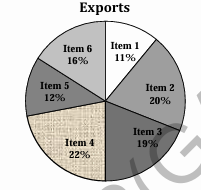
\includegraphics[width=0.5\columnwidth]{fig1.png}
    \caption{Caption} 
    \label{fig:q8} 
    \end{minipage}
    \hfill
    \begin{minipage}{0.45\textwidth}
        \centering
        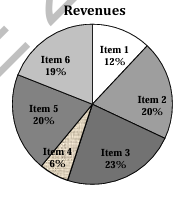
\includegraphics[width=0.5\columnwidth]{fig2.png}
        \caption{}
        \label{fig:q8}
    \end{minipage}
\end{figure}   
\hfill (GATE XL 2014)\\
    \begin{multicols}{2}
        \begin{enumerate}
            \item 1:2
            \item 2:1
            \item 1:4
            \item 4:1
        \end{enumerate}
    \end{multicols}

    \item X is 1 km northeast of Y. Y is 1 km southeast of Z. W is 1 km west of Z. P is 1 km south of W. Q is 1 km east of P. What is the distance between X and Q in km?
    \hfill (GATE XL 2014)\\
     \begin{multicols}{2}
        \begin{enumerate}
            \item 1
            \item $\sqrt{2}$
            \item $\sqrt{3}$
            \item 2
        \end{enumerate}
    \end{multicols}

    \item 10\% of the population in a town is HIV+. A new diagnostic kit for HIV detection is available; this kit correctly identifies HIV+ individuals 95\% of the time, and HIV- individuals 89\% of the time. A particular patient is tested using this kit and is found to be positive. The probability that the individual is actually positive is \underline{\hspace{2cm}}
    \hfill (GATE XL 2014)\\

\end{enumerate}
\begin{center}
    \textbf{END OF THE QUESTION PAPER}
\end{center}
\clearpage

\section*{\textbf{Chemistry (XL-H)}}

\begin{enumerate}
  \item Hybridizations of nitrogen in \ce{NO2+}, \ce{NO3-}, \ce{NH4+} respectively are:
  \hfill (GATE XL 2014)\\
  \begin{multicols}{2}
  \begin{enumerate}
    \item sp, sp2, sp3
    \item sp, sp3, sp2
    \item sp2, sp, sp3
    \item sp3, sp2, sp
  \end{enumerate}
  \end{multicols}

  \item Potassium metal crystallizes in body-centered cubic structure. The number of atoms per unit cell is: \\
  \hfill (GATE XL 2014)\\
  \begin{multicols}{2}
  \begin{enumerate}
    \item one
    \item two
    \item three
    \item four
  \end{enumerate}
  \end{multicols}

  \item Assuming ideal condition, the solution that has the highest freezing point is: \\
  \hfill (GATE XL 2014)\\
  \begin{multicols}{2}
  \begin{enumerate}
    \item 0.002 M aqueous solution of copper nitrate
    \item 0.001 M aqueous solution of potassium dichromate
    \item 0.001 M aqueous solution of sodium chloride
    \item 0.002 M aqueous solution of magnesium chloride
  \end{enumerate}
  \end{multicols}

  \item The major product formed in the following reaction is:  
  \begin{figure}[H]
      \centering
      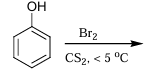
\includegraphics[width=0.34\columnwidth]{fig3.png}
      \caption{}
      \label{fig:placeholder}
  \end{figure} 
  \hfill (GATE XL 2014)\\
  \begin{multicols}{2}
  \begin{enumerate}
    \item 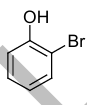
\includegraphics[width=0.2\columnwidth]{fig4.png}
    \item 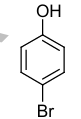
\includegraphics[width=0.2\columnwidth]{fig5.png}
    \item 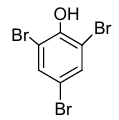
\includegraphics[width=0.2\columnwidth]{fig6.png}
    \item 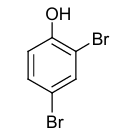
\includegraphics[width=0.2\columnwidth]{fig7.png}
  \end{enumerate}
  \end{multicols}

  \item The acid that undergoes decarboxylation most readily upon heating is: \\
  \hfill (GATE XL 2014)\\
  \begin{multicols}{2}
  \begin{enumerate}
    \item 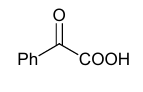
\includegraphics[width=0.2\columnwidth]{fig8.png}
    \item 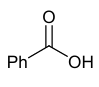
\includegraphics[width=0.2\columnwidth]{fig9.png}
    \item 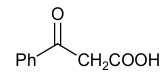
\includegraphics[width=0.3\columnwidth]{fig10.png}
    \item 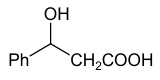
\includegraphics[width=0.3\columnwidth]{fig11.png}
  \end{enumerate}
  \end{multicols}


  \item A ball of mass 330 g is moving with a constant speed, and its associated de Broglie wavelength is 1 x 10$^{-33}$ m. The speed of the ball is \underline{\hspace{2cm}} m/s. (h = 6.6 x 10$^{-34}$)  \\
  \hfill (GATE XL 2014)\\

  \item Diphosphonic acid \ce{H4P2O5} has no P–P bond. This acid is: \\
  \hfill (GATE XL 2014)\\
  \begin{multicols}{2}
  \begin{enumerate}
    \item tetrabasic
    \item tribasic
    \item dibasic
    \item monobasic
  \end{enumerate}
  \end{multicols}

  \item The magnetic moment of an octahedral Co(II) complex is 4.0 $\mu_B$. The CFSE (in $\Delta_o$ units) is:\\
  \hfill (GATE XL 2014)\\

  \item The complex ion \ce{[Cr(H2O)6]^3+} exhibits:    \hfill (GATE XL 2014)\\
  \begin{multicols}{2}
  \begin{enumerate}
    \item slightly distorted octahedral geometry
    \item tetragonally elongated octahedral geometry
    \item tetragonally compressed octahedral geometry
    \item perfect octahedral geometry
  \end{enumerate}
  \end{multicols}

\item Assuming ideal behavior, the density of fluorine gas at $20^\circ$C and 0.3 atm is \underline{\hspace{2cm}} g L$^{-1}$. \\
\hfill (GATE XL 2014)\\
(Molecular weight of \ce{F2} = 38 g mol$^{-1}$, $R=0.082$ L atm mol$^{-1}$ K$^{-1}$)\\

\item For a first order reaction, the time required for 50\% completion is 20 minutes. The time required for 99.9\% completion of the reaction is \underline{\hspace{2cm}} minutes.\\
\hfill (GATE XL 2014)\\

\item At 298 K, the bond dissociation energies of C--H, C--C and C=C are 415, 344 and 615 kJ mol$^{-1}$, respectively. The enthalpy of atomization of carbon is 717 kJ mol$^{-1}$ and that of hydrogen is 218 kJ mol$^{-1}$. The heat of formation of naphthalene at 298 K is \underline{\hspace{2cm}} kJ mol$^{-1}$.\\
\hfill (GATE XL 2014)\\

  \item The Fischer projection that represents (2R,3S)-2,3-dihydroxybutanoic acid is: \\
  \hfill (GATE XL 2014)\\
  \begin{multicols}{2}
  \begin{enumerate}
    \item 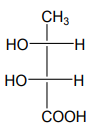
\includegraphics[width=0.3\columnwidth]{fig12.png}
    \item 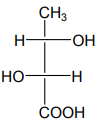
\includegraphics[width=0.3\columnwidth]{fig13.png}
    \item 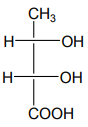
\includegraphics[width=0.3\columnwidth]{fig14.png}
    \item 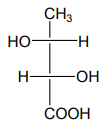
\includegraphics[width=0.3\columnwidth]{fig15.png}
  \end{enumerate}
  \end{multicols}

  \item A hydrocarbon undergoes ozonolysis to form formaldehyde and glyoxal. The compound is: \\
  \hfill (GATE XL 2014)\\
  \begin{multicols}{2}
  \begin{enumerate}
    \item 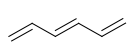
\includegraphics[width=0.3\columnwidth]{fig16.png}
    \item 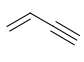
\includegraphics[width=0.3\columnwidth]{fig17.png}
    \item 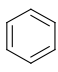
\includegraphics[width=0.2\columnwidth]{fig18.png}
    \item 
\includegraphics[width=0.3\columnwidth]{fig19.png}
  \end{enumerate}
  \end{multicols}

  \item The order of acidity of the following acids is: \\
  \hfill (GATE XL 2014)\\
  \begin{enumerate}
  \begin{multicols}{2}
      \item 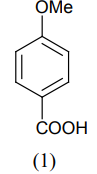
\includegraphics[width=0.3\columnwidth]{fig20.png}
      \item 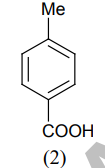
\includegraphics[width=0.3\columnwidth]{fig21.png}
      \item 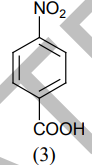
\includegraphics[width=0.3\columnwidth]{fig22.png}
      \item 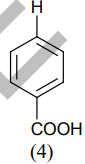
\includegraphics[width=0.3\columnwidth]{fig23.png} 
\end{multicols}
  \end{enumerate}
  \begin{multicols}{2}
  \begin{enumerate}
    \item 3 $>$ 2 $>$ 1 $>$ 4
    \item 1 $>$ 4 $>$ 3 $>$ 2
    \item 4 $>$ 3 $>$ 2 $>$ 1
    \item 3 $>$ 4 $>$ 2 $>$ 1
  \end{enumerate}
  \end{multicols}
\end{enumerate}
\begin{center}
    \textbf{END OF THE QUESTION PAPER}
\end{center}

\newpage
\section*{\textbf{Biochemistry (XL-I)}}

\begin{enumerate}
  \item During an enzyme catalyzed reaction, the equilibrium constant: 
  \hfill (GATE XL 2014)\\
  \begin{multicols}{2}
  \begin{enumerate}
    \item increases
    \item decreases
    \item remains unchanged
    \item may increase or decrease
  \end{enumerate}
  \end{multicols}

  \item A mixture of Arginine, Phenylalanine and Histidine was separated by cation exchange chromatography at pH 7. Order of elution is:
  \hfill (GATE XL 2014)\\
  \begin{multicols}{2}
  \begin{enumerate}
    \item Arg, His, Phe
    \item Phe, His, Arg
    \item His, Phe, Arg
    \item Arg, Phe, His
  \end{enumerate}
  \end{multicols}

  \item Which protease does \textbf{NOT} cleave after arginine? 
  \hfill (GATE XL 2014)\\
  \begin{multicols}{2}
  \begin{enumerate}
    \item Trypsin
    \item Proteinase K
    \item Thrombin
    \item Chymotrypsin
  \end{enumerate}
  \end{multicols}

  \item The receptor for epinephrine is:
  \hfill (GATE XL 2014)\\
  \begin{multicols}{2}
  \begin{enumerate}
    \item Tyrosine kinase receptor
    \item Serine-threonine kinase receptor
    \item G-protein coupled receptor
    \item Ligand activated transcription factor
  \end{enumerate}
  \end{multicols}

  \item Choose the option with two reducing sugars: 
  \hfill (GATE XL 2014)\\
  \begin{multicols}{2}
  \begin{enumerate}
    \item Lactose, Maltose
    \item Trehalose, Sucrose
    \item Maltose, Trehalose
    \item Lactose, Sucrose
  \end{enumerate}
  \end{multicols}

  \item The affinity of an antibody can be determined by: 
  \hfill (GATE XL 2014)\\
  \begin{multicols}{2}
  \begin{enumerate}
    \item MALDI-TOF MS
    \item Isoelectric focusing
    \item SDS-PAGE
    \item Equilibrium dialysis
  \end{enumerate}
  \end{multicols}

  \item Which molecule is an allosteric activator of PFK-1? 
  \hfill (GATE XL 2014)\\
  \begin{multicols}{2}
  \begin{enumerate}
    \item Fructose-1,6-bisphosphate
    \item Fructose-2,6-bisphosphate
    \item Glucose-6-phosphate
    \item Citrate
  \end{enumerate}
  \end{multicols}

   \item For a single substrate enzyme, a reaction is carried out at a substrate concentration four times the value of $K_{m}$. The observed initial velocity will be \underline{\hspace{2cm}} \% of $V_{\max}$.\\
   \hfill (GATE XL 2014)\\
   
   \item Consider the following biochemical reaction:  
    \[
    \text{Fructose 6-phosphate + ATP} \;\longrightarrow\; \text{Fructose 1,6-bisphosphate + ADP}
    \]  

    The equilibrium constant under biochemical standard conditions ($K'_{eq}$) for the above reaction is 254.  
    The standard free energy change ($\Delta G^{\circ'}$) for the conversion of fructose 6-phosphate is \underline{\hspace{2cm}} kJ/mol.

  \item Given below is the hydropathy plot of a monomeric transmembrane protein.
\begin{figure}[H]
    \centering
    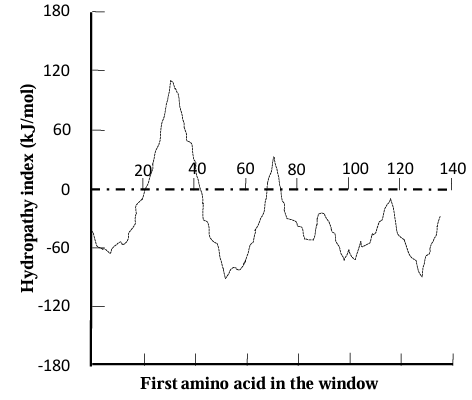
\includegraphics[width=0.5\columnwidth]{fig24.png}
    \caption{Caption}
    \label{fig:placeholder}
\end{figure}
\hfill (GATE XL 2014)\\
\begin{multicols}{2}
  \begin{enumerate}
    \item 1
    \item 2
    \item 4
    \item 5
  \end{enumerate}
  \end{multicols}

  \item An aqueous solution contains two compounds X and Y. This solution gave absorbance values of 1.0 and 0.4 at 220 and 280 nm, respectively, in a 1~cm path length cell. Molar absorption coefficients ($\varepsilon$) of the compounds X and Y are as shown in the table below. The concentration of Y in the solution is \underline{\hspace{2cm}} mM.
  \hfill (GATE XL 2014)\\

\begin{center}
\begin{tabular}{c|cc}
{} & $\varepsilon_{220}$ (M$^{-1}$cm$^{-1}$) & $\varepsilon_{280}$ (M$^{-1}$cm$^{-1}$) \\
\hline
Compound X & 1000 & 200 \\
Compound Y & 800 & 400
\end{tabular}
\end{center}
\vspace{0.5cm}

\item A purified oligomeric protein was analyzed by SDS-PAGE under reducing and non-reducing conditions. A one litre solution of 1~mg/mL concentration has $4.01 \times 10^{18}$ molecules of the oligomeric protein. Based on the data shown below, deduce the total number of polypeptide chains that constitute this protein.
\begin{figure}[H]
    \centering
    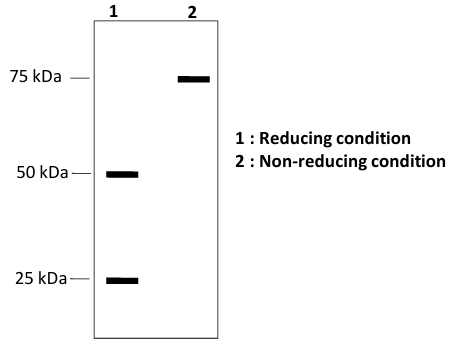
\includegraphics[width=0.5\columnwidth]{fig25.png}
    \caption{Caption}
    \label{fig:placeholder}
\end{figure}
\hfill (GATE XL 2014)\\
\begin{multicols}{2}
\begin{enumerate}
\item 2
\item 4
\item 6
\item 12
\end{enumerate}
\end{multicols}

\item The concentration of Mg$^{2+}$ ions outside a cell is twice the concentration inside. If the transmembrane potential of the cell is $-60$~mV (inside negative), the free energy change of transporting Mg$^{2+}$ ions across the membrane against the concentration gradient at $37~^{\circ}$C is \underline{\hspace{2cm}}~kJ/mol. \\
{\footnotesize (Faraday constant: 96.5~kJ/V~mol)}\\
\hfill (GATE XL 2014)\\
\item Match the entries in Group I with those in Group II:

\begin{minipage}{0.5\textwidth}
Group I
\begin{itemize}
\item[P)] J chain
\item[Q)] Serpin
\item[R)] $\beta_2$-microglobulin
\item[S)] Artemis
\end{itemize}
\end{minipage}
\begin{minipage}{0.45\textwidth}
Group II
\begin{enumerate}
\item VDJ recombinase complex
\item Component of MHC class I
\item B cell co-receptor complex
\item C1 complement inhibitor
\item Component of MHC class II
\item Multimerization of IgA and IgM
\end{enumerate}
\end{minipage}
\hfill (GATE XL 2014)\\
\begin{multicols}{2}
\begin{enumerate}
\item P-3, Q-4, R-5, S-1
\item P-6, Q-5, R-2, S-3
\item P-6, Q-4, R-2, S-1
\item P-3, Q-4, R-1, S-6
\end{enumerate}
\end{multicols}

\item The kinetic data for a single substrate enzyme is shown below. The concentration of inhibitor [I] used in the reaction was equal to the $K_i$ of the inhibitor. The $K_m$ value of an uninhibited reaction is $2 \times 10^{-5}$~M. In the presence of the inhibitor, the observed $K_m$ value is \underline{\hspace{2cm}}~$\times 10^{-5}$~M.\\
\hfill (GATE XL 2014)\\
\item One litre of phosphate buffer was prepared by adding 208~g of Na$_2$HPO$_4$ (Mol. wt. 142) and 71~g of NaH$_2$PO$_4$ (Mol. wt. 120) in water. If the p$K_a$ for the dissociation of H$_2$PO$_4^-$ into HPO$_4^{2-}$ and H$^+$ is 6.86, the pH of the buffer will be \underline{\hspace{2cm}}.\\
\hfill (GATE XL 2014)\\
\item Shown below is an electrospray ionization mass spectrum of a protein. 
\begin{figure}[H]
    \centering
    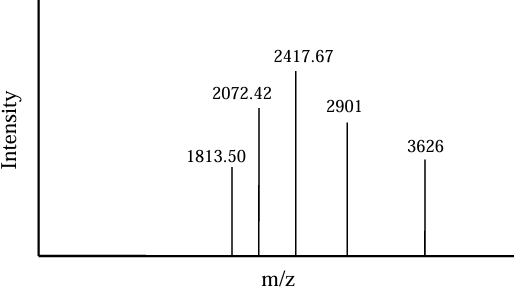
\includegraphics[width=0.5\columnwidth]{fig26.png}
    \caption{Caption}
    \label{fig:placeholder}
\end{figure}

The numbers on top of the peaks are the m/z values. The mass of the protein deduced from the given data is \underline{\hspace{2cm}}~kDa.\\
\hfill (GATE XL 2014)\\
\item A human gene has only three exons (I, II, and III in the given order). Total RNA was isolated from cultured human kidney cells and reverse transcribed. The resultant cDNA was used as a template in a PCR reaction containing a forward primer specific to Exon I and a reverse primer specific to Exon III. When the PCR product was analyzed by gel electrophoresis, two bands were observed of sizes 2.5~kb and 1~kb. However, when Northern blotting was performed with the same total RNA using a radiolabeled probe specific to Exon II, only one band was observed. Based on these observations, which one of the following statements is \textbf{FALSE}?
\hfill (GATE XL 2014)\\
\begin{enumerate}
\item Northern blotting with a probe specific to Exon III will show two bands.
\hfill (GATE XL 2014)\\
\item The gene codes for two mRNA splice variants.
\item If the forward primer were specific to Exon II, two bands will be observed.
\item The Exon II is 1.5~kb in size.
\end{enumerate}

\item Using Sanger’s dideoxy chain termination method, a particular exonic region of a protein coding gene was sequenced for two individuals (Subject 1 and Subject 2). The figure shows a segment of the autoradiogram corresponding to a small window of the DNA sequence. Which one of the following interpretations is correct for the sequenced DNA fragments?
\begin{figure}[H]
    \centering
    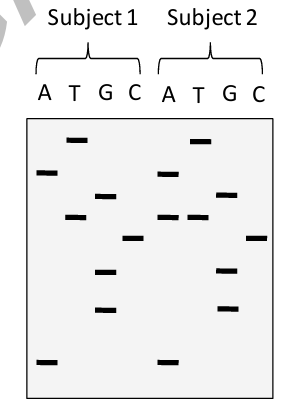
\includegraphics[width=0.3\columnwidth]{fig27.png}
    \caption{}
    \label{fig:placeholder}
\end{figure}
\hfill (GATE XL 2014)\\
\begin{enumerate}
\item Subject 2 has two allelic variants.
\item Subject 1 has the sequence 5'-TAGTCGGA-3'.
\item Subject 2 has the sequence 5'-AGGCTAGAT-3'.
\item Subject 1 has a single nucleotide deletion in the gene.
\end{enumerate}
\vspace{0.5cm}

\item A 7~kb DNA molecule of a specific sequence has two EcoRI and one PvuII restriction endonuclease sites. The restriction sites are shown below. The DNA was completely digested with both EcoRI and PvuII. The digestion product was purified and added to an appropriately buffered reaction mixture at 37$^\circ$C, which contained the Klenow fragment of DNA polymerase~I and $\alpha$-\textsuperscript{32}P~dNTPs. After one hour, the DNA in the reaction product was purified and analyzed by electrophoresis. The bands were visualized by both ethidium bromide (EtBr) staining and autoradiography. The result is shown below. Which one of the following restriction maps is in agreement with the above result?
\begin{figure}[H]
    \centering
    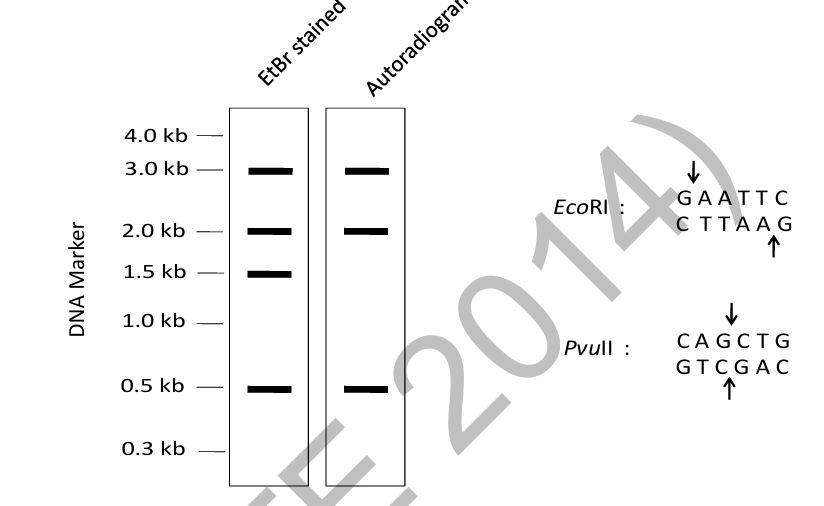
\includegraphics[width=0.5\columnwidth]{fig28.png}
    \caption{Caption}
    \label{fig:placeholder}
\end{figure}
\hfill (GATE XL 2014)\\
\begin{multicols}{2}
\begin{enumerate}
\item 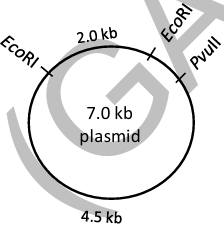
\includegraphics[width=0.4\columnwidth]{fig29.png}
\item 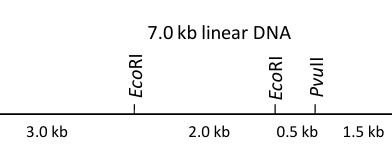
\includegraphics[width=0.5\columnwidth]{fig30.png}
\item 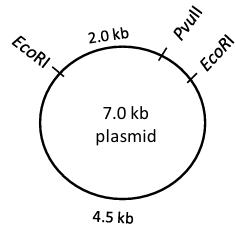
\includegraphics[width=0.4\columnwidth]{fig31.png}
\item 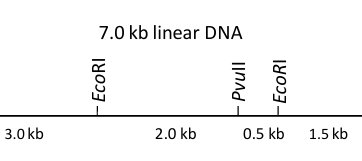
\includegraphics[width=0.5\columnwidth]{fig32.png}
\end{enumerate}
\end{multicols}

\end{enumerate}
\begin{center}
    \textbf{END OF THE QUESTION PAPER}
\end{center}
\clearpage

\section*{{Botany Section}}
\begin{enumerate}

\item Plant which grows attached to another plant species but is not a parasitic is known as \hfill(GATE XL 2014)\\
\begin{multicols}{2}
\begin{enumerate}
\item Endophyte
\item Halophyte
\item Epiphyte
\item Lithophyte
\end{enumerate}
\end{multicols}

\item An ideal cybrid should have \hfill(GATE XL 2014)\\
\begin{multicols}{2}
\begin{enumerate}
\item both nuclear genome and cytoplasmic genome equally from both the parents
\item nuclear genome from one of the parents and cytoplasmic genome from other parent
\item nuclear genome predominantly/exclusively from one of the parents and cytoplasmic genome equally from both the parents
\item nuclear genome equally from both the parents and cytoplasmic genome predominantly/ exclusively from one of the parents
\end{enumerate}
\end{multicols}

\item Transmission Electron Micrograph of fungal cell can usually be distinguished from plant cell due to lack of P and having less abundant Q. Find the correct combination of P and Q. \hfill(GATE XL 2014)\\
\begin{multicols}{2}
\begin{enumerate}
\item P- Plastid; Q-Vacuoles
\item P- Plastid; Q-Mitochondria
\item P- Plastid; Q-Endoplasmic reticulum
\item P- Mitochondria; Q-Plastid
\end{enumerate}
\end{multicols}

\item Identify the \textbf{CORRECT} answer\\
RNA interference (RNAi) \\
P. is an event of post transcriptional gene silencing\\
Q. works through RNA induced silencing complex \hfill(GATE XL 2014)\\
\begin{multicols}{2}
\begin{enumerate}
\item P only
\item Q only
\item Both P and Q
\item neither P nor Q
\end{enumerate}
\end{multicols}

\item Find the odd one out \hfill(GATE XL 2014)\\
\begin{multicols}{2}
\begin{enumerate}
\item Petal
\item Sepal
\item Petiole
\item Tepal
\end{enumerate}
\end{multicols}

\item \textbf{Plantibody} is the \hfill(GATE XL 2014)\\
\begin{multicols}{2}
\begin{enumerate}
\item \textbf{Antibody} expressed in transgenic plant
\item \textbf{Transgenic plant} that expresses antibody
\item \textbf{Antibody} against plant based antigen
\item \textbf{Transgenic plant} that expresses antigen
\end{enumerate}
\end{multicols}

\item In a typical oil-seed crop, the matured seeds are enriched with \hfill(GATE XL 2014)\\
\begin{multicols}{2}
\begin{enumerate}
\item Phospholipid
\item Galactolipid
\item Neutral lipid
\item Sphingolipid
\end{enumerate}
\end{multicols}

\item Match the following products (Column I) with the corresponding plant species (Column II): \hfill(GATE XL 2014)\\
Column I: P. Saffron, Q. Gamboge, R. Litmus, S. Turmeric\\
Column II: 1. Garcinia sp., 2. Rocella tinctoria, 3. Crocus sativus, 4. Curcuma sp.\\
\begin{multicols}{2}
\begin{enumerate}
\item P-4, Q-2, R-1, S-3
\item P-3, Q-4, R-1, S-2
\item P-2, Q-3, R-2, S-1
\item P-3, Q-1, R-2, S-4
\end{enumerate}
\end{multicols}

\item The semi-dwarf trait of corn, wheat and rice plants used in breeding program during 1960s resulted in green revolution. Later this ‘green-revolution gene’ has been identified to be involved in either signal transduction pathway or biosynthesis of \hfill(GATE XL 2014)\\
\begin{multicols}{2}
\begin{enumerate}
\item Auxin
\item Gibberellin
\item Cytokinin
\item Ethylene
\end{enumerate}
\end{multicols}

\item In classical model to explain the plant-pathogen interaction, the host will not develop the disease upon the pathogen attack when \hfill(GATE XL 2014)\\
\begin{multicols}{2}
\begin{enumerate}
\item The resistance gene (R) is non-functional
\item The avirulence gene (Avr) is non-functional
\item Both R and Avr are non-functional
\item Both R and Avr are functional
\end{enumerate}
\end{multicols}

    \item Select the CORRECT combination from the promoter (Column I), transcription machinery used (Column II) and target tissue type (Column III) to express a foreign gene in a plant system.  

    \begin{tabular}{lll}
    Column I & Column II & Column III \\
    P. Ubiquitin & 1. Chloroplast & i. Leaf \\
    Q. Napin & 2. Nucleus & ii. Seed \\
    R. RbcL & 3. Mitochondria & \\
    S. RbcS & & \\
    \end{tabular}\\
    \hfill (GATE XL 2014)
    \begin{multicols}{2}
    \begin{enumerate}
        \item P-1-i, Q-3-ii, R-2-i, S-3-ii  
        \item P-3-i, Q-1-i, R-2-ii, S-1-ii  
        \item P-2-i, Q-2-ii, R-1-i, S-2-i  
        \item P-1-ii, Q-3-i, R-2-ii, S-3-ii  
    \end{enumerate}
    \end{multicols}

    \item In a plant species, flower colour purple is dominant over white. One such purple-flowered plant upon selfing produced 35 viable plants, of which 9 were white-flowered and the rest were purple-flowered. What fraction of these purple-flowered progeny is expected to be pure purple-flowered line?  \\
    \hfill (GATE XL 2014)
    \begin{multicols}{2}
    \begin{enumerate}
        \item $\tfrac{1}{2}$  
        \item $\tfrac{1}{3}$  
        \item $\tfrac{1}{4}$  
        \item $\tfrac{2}{3}$  
    \end{enumerate}
    \end{multicols}


    \item Following diagram represents the sequence of genes in a normal chromosome of a plant species. Match the CORRECT combination for chromosomal mutation using Column I and Column II.  

    \begin{tabular}{ll}
    Column I & Column II \\
    P.GHIKL JMN & 1. Tandem duplication \\
    Q.GJ KLHIMN & 2. Deletion \\
    R.GHIJ KLKLMN & 3. Pericentric inversion \\
    S.GHJ KLMN & 4. Non-reciprocal translocation \\
    \end{tabular}\\
    \hfill (GATE XL 2014)
    \begin{multicols}{2}
    \begin{enumerate}
        \item P-4, Q-3, R-2, S-1  
        \item P-1, Q-3, R-4, S-2  
        \item P-2, Q-1, R-4, S-3  
        \item P-3, Q-4, R-1, S-2  
    \end{enumerate}
    \end{multicols}

    \item Match the nuclei status of mutant plant (Column I) with the typical chromosome number (Column II), when the wild type plant species is having 2N = 46 chromosomes.  

    \begin{tabular}{ll}
    Column I & Column II \\
    P. Trisomic & 1. 23 \\
    Q. Triploid & 2. 45 \\
    R. Monosomic & 3. 47 \\
    S. Monoploid & 4. 69 \\
    \end{tabular}\\
    \hfill (GATE XL 2014)
    \begin{multicols}{2}
    \begin{enumerate}
        \item P-1, Q-2, R-3, S-4  
        \item P-2, Q-3, R-4, S-1  
        \item P-3, Q-4, R-2, S-1  
        \item P-4, Q-3, R-1, S-2  
    \end{enumerate}
    \end{multicols}

    \item Match the following reporter genes used in plant transformation experiments with the source of gene and detection/assay system.  

    \begin{tabular}{lll}
    Reporter gene & Source & Detection/assay \\
    P. $\beta$-glucuronidase & 3. E. coli & i. Radioactive assay \\
    Q. Green fluorescence protein & 1. Aequorea victoria & ii. Fluorimetric \\
    R. Luciferase & 2. Photinus pyralis & iii. Fluorescence \\
    S. Chloramphenicol acetyl transferase &  & iv. Luminescence \\
    \end{tabular}\\
    \hfill (GATE XL 2014)
    \begin{multicols}{2}
    \begin{enumerate}
        \item P-3-i, Q-1-ii, R-2-iii, S-3-iv  
        \item P-3-ii, Q-1-iii, R-2-iv, S-3-i  
        \item P-2-ii, Q-1-iii, R-3-iv, S-1-i  
        \item P-1-ii, Q-2-iii, R-3-i, S-3-iv  
    \end{enumerate}
    \end{multicols}

    \item Find the CORRECT statements in the context of Global warming effect on plant photosynthesis.  \\
    \hfill (GATE XL 2014)
    \begin{multicols}{2}
    \begin{enumerate}
        \item P \& Q  
        \item R \& S  
        \item P \& R  
        \item P \& S  
    \end{enumerate}
    \end{multicols}


    \item Statements given below are either TRUE (T) or FALSE (F). Find the correct combination.  \\
    \hfill (GATE XL 2014)
    \begin{multicols}{2}
    \begin{enumerate}
        \item P-T, Q-F, R-T, S-F  
        \item P-T, Q-T, R-T, S-F  
        \item P-T, Q-F, R-F, S-T  
        \item P-T, Q-F, R-T, S-T  
    \end{enumerate}
    \end{multicols}

    \item Match the following diagrams P, Q, R, and S with the inflorescence type (Column I) and the corresponding plant species (Column II).  
    \begin{figure}[H]
        \centering
        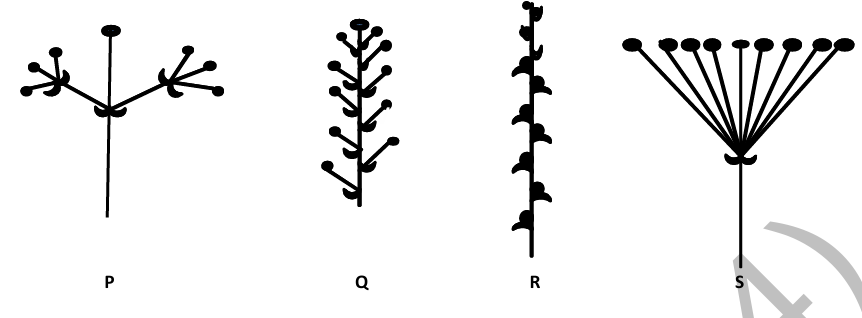
\includegraphics[width=0.5\columnwidth]{fig33.png}
        \caption{}
        \label{fig:placeholder}
    \end{figure}

    \begin{tabular}{ll}
    Column I & Column II \\
    1. Umbel & i. Pedicularis sp. \\
    2. Raceme & ii. Smilacina sp. \\
    3. Compound determinate & iii. Epilobium sp. \\
    4. Spike & iv. Pelargonium sp. \\
    \end{tabular}\\
    \hfill (GATE XL 2014)
    \begin{multicols}{2}
    \begin{enumerate}
        \item P-2-i, Q-3-iv, R-4-ii, S-1-iii  
        \item P-3-ii, Q-2-iii, R-4-i, S-1-iv  
        \item P-1-iii, Q-3-ii, R-4-iv, S-2-i  
        \item P-1-iv, Q-4-i, R-2-iii, S-3-ii  
    \end{enumerate}
    \end{multicols}


    \item Find the right combination for P, Q, R and S with respect to gametophyte development in flowering plants.  
   \hfill (GATE XL 2014)
   \begin{figure}[H]
       \centering
       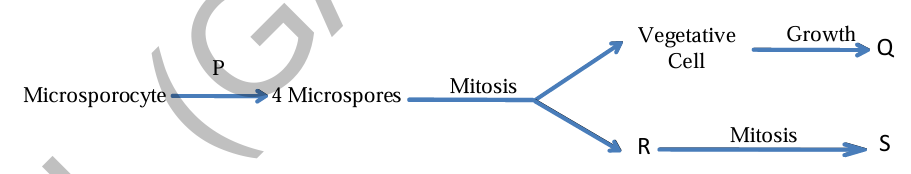
\includegraphics[width=0.9\columnwidth]{fig34.png}
       \caption{Caption}
       \label{fig:placeholder}
   \end{figure}
    \begin{multicols}{2}
    \begin{enumerate}
        \item P-Meiosis, Q-Generative cell, R-Pollen Tube, S-2 Sperm Cells  
        \item P-Meiosis, Q-Pollen Tube, R-Generative Cell, S-2 Sperm Cells  
        \item P-Mitosis, Q-Generative Cell, R-Pollen Tube, S-2 Sperm Cells  
        \item P-Growth, Q-2 Sperm Cells, R-Pollen Tube, S-Generative Cell  
    \end{enumerate}
    \end{multicols}


    \item Match the definition (Column I) with the type of plant community (Column II).  

    \begin{tabular}{ll}
    Column I & Column II \\
    P. Occupation of an area by plant communities to maturity & 1. Formation \\
    Q. A major ecological unit of vegetation & 2. Consociation \\
    R. A smaller unit of plant association & 3. Faciation \\
    S. Subdivision of plant association (minor temp/moisture) & 4. Plant succession \\
    \end{tabular}\\
   \hfill (GATE XL 2014)
    \begin{multicols}{2}
    \begin{enumerate}
        \item P-1, Q-3, R-4, S-2  
        \item P-3, Q-2, R-1, S-4  
        \item P-4, Q-1, R-2, S-3  
        \item P-2, Q-4, R-3, S-1  
    \end{enumerate}
    \end{multicols}
\end{enumerate}
\begin{center}
    \textbf{END OF THE QUESTION PAPER}
\end{center}
\clearpage

\section*{Microbiology Section}

\begin{enumerate}

\item Most viral capsids have 
\hfill(GATE XL 2014)
\begin{multicols}{2}
\begin{enumerate}
\item 08 faces
\item 12 faces
\item 16 faces
\item 20 faces
\end{enumerate}
\end{multicols}

\item Intergenic suppression involves mutation in \hfill(GATE XL 2014)
\begin{multicols}{2}
\begin{enumerate}
\item rRNA
\item mRNA
\item tRNA
\item cDNA
\end{enumerate}
\end{multicols}

\item Which one of the following proteins does \textbf{NOT} bind to a gaseous ligand? \hfill(GATE XL 2014)\\
\begin{multicols}{2}
\begin{enumerate}
\item Leghemoglobin
\item Carbonic anhydrase
\item Nitrogenase
\item NADPH oxidase
\end{enumerate}
\end{multicols}

\item A bacterial culture ($5 \times 10^8$ cells/ml) is maintained in a chemostat of working volume 10 L. If the doubling time of the bacteria is 50 min, the required rate of flow of nutrients (in ml/min) is \rule{2cm}{0.1pt}. \hfill(GATE XL 2014)\\

\item Rheumatic fever is an example of \hfill(GATE XL 2014)
\begin{multicols}{2}
\begin{enumerate}
\item autoimmune disease
\item type IV hypersensitive reaction
\item immunodeficiency disease
\item neurodegenerative disorder
\end{enumerate}
\end{multicols}

\item Oxygenases that catalyse the initial step in the degradation of polycyclic aromatic hydrocarbons by using molecular oxygen belong to which enzyme class? \hfill(GATE XL 2014)
\begin{multicols}{2}
\begin{enumerate}
\item Hydrolase
\item Transferase
\item Lyase
\item Oxido-reductase
\end{enumerate}
\end{multicols}

\item Which one of the following is \textbf{NOT}     involved in horizontal gene transfer? \hfill(GATE XL 2014)
\begin{multicols}{2}
\begin{enumerate}
\item Conjugation
\item Transformation
\item Transduction
\item Mutation
\end{enumerate}
\end{multicols}

\item The principle of immunization was first explained by \hfill(GATE XL 2014)
\begin{multicols}{2}
\begin{enumerate}
\item Edward Jenner
\item Elie Metchnikoff
\item Louis Pasteur
\item Robert Koch
\end{enumerate}
\end{multicols}

\item Lysozyme catalyzes the breakdown of \hfill(GATE XL 2014)
\begin{multicols}{2}
\begin{enumerate}
\item NAG-NAM
\item lipopolysaccharide
\item teichoic acid
\item lipoprotein A
\end{enumerate}
\end{multicols}

\item Which one of the following microscopic techniques can be used to study the contour of proteins? \hfill(GATE XL 2014)
\begin{multicols}{2}
\begin{enumerate}
\item SEM
\item TEM
\item AFM
\item Confocal microscopy
\end{enumerate}
\end{multicols}

    \item Match compounds in Group I with inhibitory activities in Group II.  

    \begin{tabular}{ll}
    Group I & Group II \\
    (P) Vancomycin & (i) Folate metabolism \\
    (Q) Rifampin & (ii) DNA synthesis \\
    (R) Puromycin & (iii) Protein synthesis \\
    (S) Ciprofloxacin & (iv) RNA synthesis \\
                      & (v) Cell wall synthesis \\
    \end{tabular}
    \hfill (GATE XL 2014)
    \begin{multicols}{2}
    \begin{enumerate}
        \item P-v, Q-iv, R-iii, S-ii  
        \item P-iv, Q-iii, R-i, S-ii  
        \item P-iv, Q-i, R-iii, S-ii  
        \item P-v, Q-iii, R-ii, S-iv  
    \end{enumerate}
    \end{multicols}


    \item Match the organisms with the appropriate growth curves.  

    \begin{tabular}{l}
    (P) Bacteria \\
    (Q) Extracellular virus \\
    (R) Intracellular virus \\
    \end{tabular}
    \begin{figure}[H]   
        \centering
        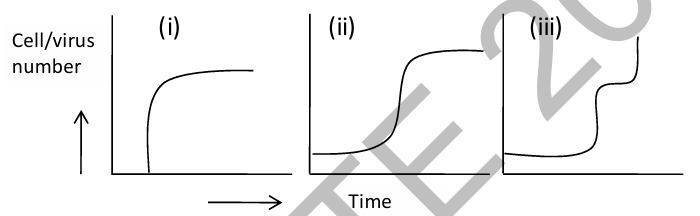
\includegraphics[width=0.5\columnwidth]{fig35.png}
        \caption{}
        \label{fig:placeholder}
    \end{figure}
    \hfill (GATE XL 2014)
    \begin{multicols}{2}
    \begin{enumerate}
        \item P-iii, Q-i, R-ii  
        \item P-ii, Q-i, R-iii  
        \item P-ii, Q-iii, R-i  
        \item P-i, Q-ii, R-iii  
    \end{enumerate}
    \end{multicols}


    \item The length of a coding region in an mRNA is 897 bases.  
    How many amino acids will be there in the polypeptide synthesized using this mRNA?  
    \hfill (GATE XL 2014)
    \begin{multicols}{2}
    \begin{enumerate}
        \item 297  
        \item 298  
        \item 299  
        \item 897  
    \end{enumerate}
    \end{multicols}


    \item Match the media in Group I for screening microbial isolates in Group II.  

    \begin{tabular}{ll}
    Group I & Group II \\
    (P) Blood agar media & (i) Coliforms \\
    (Q) Minimal media & (ii) Protease producers \\
    (R) Skimmed milk agar media & (iii) Hemolytic microbes \\
    (S) Bile salt media & (iv) Lipase producers \\
                        & (v) Autotrophs \\
    \end{tabular}
    \hfill (GATE XL 2014)
    \begin{multicols}{2}
    \begin{enumerate}
        \item P-iii, Q-v, R-ii, S-i  
        \item P-iii, Q-ii, R-i, S-iv  
        \item P-i, Q-iii, R-ii, S-iv  
        \item P-ii, Q-i, R-iv, S-v  
    \end{enumerate}
    \end{multicols}


    \item During a bacterial growth experiment, the total viable cell count at 2 h and 6 h was  
    $1\times10^4$ cells/ml and $1\times10^9$ cells/ml, respectively.  
    The specific growth rate (in h$^{-1}$) of the culture is \underline{\hspace{2cm}}. 
    \hfill (GATE XL 2014)

    \item The concentration of sodium chloride in the cytoplasm of a *Halobacterium* sp. was found  
    to be 250 ng/nl. The molarity (in M) of sodium chloride is \underline{\hspace{2cm}}.  
    \hfill (GATE XL 2014)\\

    \item Match organisms in Group I with shapes in Group II and flagellar arrangements in Group III.  

    \begin{tabular}{lll}
    Group I & Group II & Group III \\
    (P) Salmonella typhi & (i) Helical & (1) Non-motile \\
    (Q) Saccharomyces cerevisiae & (ii) Rod & (2) Amphitrichous \\
    (R) Aquaspirillum serpens & (iii) Curved rod & (3) Peritrichous \\
    (S) Vibrio cholerae & (iv) Ovoid & (4) Polar \\
    \end{tabular}
   \hfill (GATE XL 2014)
    \begin{multicols}{2}
    \begin{enumerate}
        \item P-ii-3, Q-iv-1, R-i-2, S-iii-4  
        \item P-iii-1, Q-iv-2, R-ii-4, S-i-3  
        \item P-i-2, Q-ii-4, R-iii-2, S-iv-3  
        \item P-ii-2, Q-iii-1, R-i-3, S-iv-4  
    \end{enumerate}
    \end{multicols}
 

    \item Lethal dose curves of different microorganisms (1, 2, 3 and 4) are shown below.  
    Which of these organisms is most pathogenic?  
\begin{figure}[H]
    \centering
    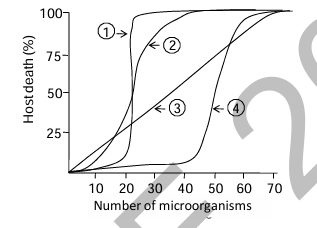
\includegraphics[width=0.5\columnwidth]{fig36.png}
    \caption{}
    \label{fig:placeholder}
\end{figure}   
\hfill (GATE XL 2014)
\begin{enumerate}
\begin{multicols}{2}
    \item 1 and 3 only
    \item 1 and 2 only
    \item 3 and 4 only
    \item 2 and 3 only
\end{multicols}
\end{enumerate}


    \item The 16S rRNA sequence is widely used in bacterial systematics because it is
    \hfill (GATE XL 2014) 
    \begin{multicols}{2}
    \begin{enumerate}
        \item Highly conserved  
        \item Short length  
        \item Unique to each strain  
        \item Encoded by plasmids  
    \end{enumerate}
    \end{multicols}


    \item Which of the following methods is best suited to isolate pure colonies from a mixed bacterial culture?  \\
    \hfill (GATE XL 2014)
    \begin{multicols}{2}
    \begin{enumerate}
        \item Pour plate method  
        \item Streak plate method  
        \item Spread plate method  
        \item Roll tube method  
    \end{enumerate}
    \end{multicols}
 \begin{center}
     \textbf{END OF THE QUESTION PAPER}
 \end{center}

\end{enumerate}
\newpage
\section*{Zoology Section}

\begin{enumerate}

\item Small geographic areas with high concentrations of endemic species and a large number of endangered and threatened species are known as \hfill(GATE XL 2014)\\
\begin{multicols}{2}
\begin{enumerate}
\item endemic sinks
\item critical communities
\item biodiversity hot spots
\item endemic metapopulations
\end{enumerate}
\end{multicols}

\item Which ONE of the following animals has "Osculum" as an excretory structure? \hfill(GATE XL 2014)\\
\begin{multicols}{2}
\begin{enumerate}
\item Hydra
\item Sponge
\item Jelly Fish
\item Sea pen
\end{enumerate}
\end{multicols}

\item During development of which ONE of the following organisms, bilateral meroblastic cleavage is found? \hfill(GATE XL 2014)\\
\begin{multicols}{2}
\begin{enumerate}
\item Mollusc
\item Fish
\item Bird
\item Amphibian
\end{enumerate}
\end{multicols}

\item The mitochondrion is NOT considered a part of the endomembrane system on account of which ONE of the following reasons? \hfill(GATE XL 2014)\\
\begin{multicols}{2}
\begin{enumerate}
\item It does not undergo structural changes
\item It is not derived from the ER or Golgi
\item It does not synthesize proteins
\item It is not attached to the outer nuclear envelope
\end{enumerate}
\end{multicols}

\item The end products of glycolysis include ATP, \hfill(GATE XL 2014)\\
\begin{multicols}{2}
\begin{enumerate}
\item CO$_{2}$ and H$_{2}$O
\item H$_{2}$O and pyruvate
\item NADH and pyruvate
\item CO$_{2}$ and NADH
\end{enumerate}
\end{multicols}

\item The TATA box is found in the vicinity of the transcription start site. The role of this box is to \hfill(GATE XL 2014)\\
\begin{multicols}{2}
\begin{enumerate}
\item serve as a ribosome recruitment site
\item serve as RNA polymerase binding site
\item provide 3-D structural integrity to a DNA molecule
\item act as a terminator sequence
\end{enumerate}
\end{multicols}

\item Which ONE of the following processes does NOT occur in prokaryotic gene expression, but occurs in eukaryotic gene expression? \hfill(GATE XL 2014)\\
\begin{multicols}{2}
\begin{enumerate}
\item Transcription of mRNA, tRNA, and rRNA
\item Binding of RNA polymerase to the promoter
\item Addition of a poly-A tail to the 3' end and the 5' capping of an mRNA
\item Translation begins as soon as transcription is initiated
\end{enumerate}
\end{multicols}

\item In Graves’ disease, the presence of auto antibodies against which ONE of the following molecules is the direct cause of hyperthyroidism? \hfill(GATE XL 2014)\\
\begin{multicols}{2}
\begin{enumerate}
\item Thyroperoxidase
\item Thyroxine
\item Thyroid stimulating hormone
\item Thyroid stimulating hormone receptor
\end{enumerate}
\end{multicols}

\item In mammals, the two important organs associated with the production and elimination of urea are \hfill(GATE XL 2014)\\
\begin{multicols}{2}
\begin{enumerate}
\item gastrointestinal tract and lungs
\item gastrointestinal tract and liver
\item kidneys and lungs
\item liver and kidneys
\end{enumerate}
\end{multicols}

\item Some endocrine glands produce hormones that stimulate functions of other endocrine glands. Which ONE of the following hormones specifically acts to increase secretion of other hormones? \hfill(GATE XL 2014)\\
\begin{multicols}{2}
\begin{enumerate}
\item Thyroxine
\item Prolactin
\item ACTH
\item ADH
\end{enumerate}
\end{multicols}

\item If the recombination frequency between X - Y loci is 12, X - Z loci is 4, and Y - Z loci is 8, then the order of the loci on the chromosome is \hfill(GATE XL 2014)\\
\begin{multicols}{2}
\begin{enumerate}
\item X-Y-Z
\item Y-X-Z
\item X-Z-Y
\item Z-Y-X
\end{enumerate}
\end{multicols}

\item A cross is made between a white eyed-miniature winged female with a red eyed-normal winged male of \textit{Drosophila melanogaster}. Further crossing of F1 female offspring from this cross with a white eyed-miniature winged male fly gave 95 white eyed-normal winged, 102 red eyed-miniature winged, 226 red eyed-normal winged, and 202 white eyed-miniature winged offspring in F2 generation. What is the percent frequency of recombination between the two genes? \hfill(GATE XL 2014)\\
\begin{multicols}{2}
\begin{enumerate}
\item 20.11
\item 31.52
\item 49.10
\item 34.12
\end{enumerate}
\end{multicols}

\item A green fluorescent protein (GFP) encoding gene is fused to a gene encoding specific protein for expression in cells. What is the advantage of using GFP over staining cells with fluorescently labeled antibodies that bind to the target protein? \hfill(GATE XL 2014)\\
\begin{enumerate}
\item It bleaches less compared to fluorescent probes
\item It allows imaging at higher resolution than fluorescent probes
\item It provides more precise location of the protein than fluorescent probes
\item Its fusion allows tracking the location of the protein in living cells, while staining usually requires fixation of cells
\end{enumerate}

\item A newborn was accidentally given a drug that destroyed the thymus. Which ONE of the following would be the most likely outcome? \hfill(GATE XL 2014)\\
\begin{multicols}{2}
\begin{enumerate}
\item Lack of class I MHC molecules
\item Inability to rearrange antigen receptors
\item Inability to differentiate to mature T cells
\item Reduction in T-independent number of B cells
\end{enumerate}
\end{multicols}

\item One individual has a parasitic worm infection and another is responding to an allergen such as pollen. Which ONE of the following features is common to both of them? \hfill(GATE XL 2014)\\
\begin{multicols}{2}
\begin{enumerate}
\item Increase in cytotoxic T cell population
\item Risk of developing an autoimmune disease
\item Reduced innate immune response
\item Increased levels of IgE
\end{enumerate}
\end{multicols}

\item Five dialysis bags (DB1-DB5), impermeable to sucrose, were filled with various concentrations of sucrose. The bags were placed in separate beakers containing 0.6 M sucrose solution. Every 10 minutes, the bags were weighed and the percent change in mass of each bag was plotted as a function of time. \\
\begin{figure}[H]
    \centering
    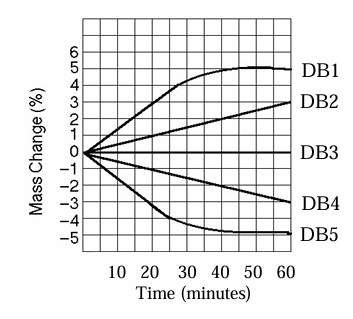
\includegraphics[width=0.5\columnwidth]{fig37.png}
    \caption{}
    \label{fig:placeholder}
\end{figure}
Which plot in the graph represent(s) bags containing a solution that is hypertonic at 50 minutes? \hfill(GATE XL 2014)\\
\begin{multicols}{2}
\begin{enumerate}
\item DB2
\item DB4
\item DB3
\item DB4 and DB5
\end{enumerate}
\end{multicols}

\item Which ONE of the following combinations of products will result, when 3 molecules of acetyl CoA is fed into TCA cycle? \hfill(GATE XL 20184)\\
\begin{multicols}{2}
\begin{enumerate}
\item 1 ATP, 2 CO$_2$, 3 NADH, and 1 FADH$_2$
\item 3 ATP, 6 CO$_2$, 9 NADH, and 3 FADH$_2$
\item 3 ATP, 3 CO$_2$, 3 NADH, and 3 FADH$_2$
\item 38 ATP, 6 CO$_2$, 3 NADH, and 12 FADH$_2$
\end{enumerate}
\end{multicols}

\item A DNA fragment shown below has restriction sites I and II, which create fragments X, Y, and Z. Which ONE of the following agarose gel electrophoresis patterns represents the separation of these fragments? \hfill(GATE XL 2014)\\
\begin{figure}[H]
    \centering
    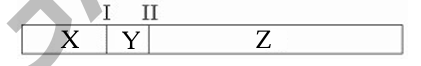
\includegraphics[width=0.5\columnwidth]{fig38.png}
    \caption{}
    \label{fig:placeholder}
\end{figure}
\begin{multicols}{2}
\begin{enumerate}
\item 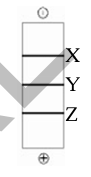
\includegraphics[width=0.2\columnwidth]{fig39.png}
\item 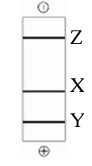
\includegraphics[width=0.2\columnwidth]{fig40.png}
\item 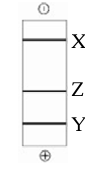
\includegraphics[width=0.2\columnwidth]{fig41.png}
\item 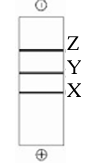
\includegraphics[width=0.2\columnwidth]{fig42.png}
\end{enumerate}
\end{multicols}

\item Theoretically, it is possible to resurrect the extinct woolly mammoth by which ONE of the following methods? \hfill(GATE XL 2014)\\
\begin{multicols}{2}
\begin{enumerate}
\item Transferring cell nuclei from the frozen tissue into enucleated unfertilized eggs of a suitable mammal
\item Introducing sequenced mammoth genome into donor eggs of a suitable mammal
\item Transferring mammoth nuclear material into stem cells
\item Collection of oocytes from ovaries of the frozen mammoth for in vitro fertilization and transfer of fertilized eggs into animals such as elephants
\end{enumerate}
\end{multicols}

\item Regions of higher abundance of cholesterol molecules on the plasma membrane will \hfill(GATE XL 2014)\\
\begin{multicols}{2}
\begin{enumerate}
\item be more fluid
\item result in clogged arteries as it can detach from the plasma membrane
\item be more rigid than the surrounding membrane
\item have higher rates of lateral movement of proteins into and out of plasma membrane
\end{enumerate}
\end{multicols}

\end{enumerate}
\begin{center}
    \textbf{END OF THE QUESTION PAPER}
\end{center}
\newpage
\section*{Food Technology}
\begin{enumerate}
    \item Which one of the following is NOT a source of caffeine?  
    \hfill (GATE XL 2014)
    \begin{multicols}{2}
    \begin{enumerate}
        \item Coffee  
        \item Cocoa beans  
        \item Corn syrup  
        \item Tea leaves  
    \end{enumerate}
    \end{multicols}
    

    \item Yoghurt is prepared using a pair of microorganisms. Choose the correct pair from the following:  
    \hfill (GATE XL 2014)
    \begin{multicols}{2}
    \begin{enumerate}
        \item \textit{Lactobacillus bulgaricus}, \textit{Streptococcus thermophilus}  
        \item \textit{Lactobacillus lactis}, \textit{Streptococcus thermophilus}  
        \item \textit{Lactobacillus bulgaricus}, \textit{Streptococcus lactis}  
        \item \textit{Lactobacillus lactis}, \textit{Streptococcus lactis}  
    \end{enumerate}
    \end{multicols}
    

    \item Choose the target organism for milk pasteurization from the following:  
    \hfill (GATE XL 2014)
    \begin{multicols}{2}
    \begin{enumerate}
        \item \textit{Mycobacterium tuberculosis}  
        \item \textit{Coxiella burnetii}  
        \item \textit{Clostridium botulinum}  
        \item \textit{Bacillus cereus}  
    \end{enumerate}
    \end{multicols}
    

    \item Hypobaric storage is also known as \underline{\hspace{3cm}} 
    \hfill (GATE XL 2014)
    \begin{multicols}{2}
    \begin{enumerate}
        \item Modified atmospheric storage  
        \item Controlled atmospheric storage  
        \item Low pressure storage  
        \item Modified aseptic package  
    \end{enumerate}
    \end{multicols}
 

    \item In a solution of vegetable oil (molecular mass = 292 kg kmol$^{-1}$) and ethanol (molecular mass = 46 kg kmol$^{-1}$), the concentration of vegetable oil in the solution is measured to be 60\% (total mass basis). Therefore, mole fraction of ethanol in the solution is \underline{\hspace{3cm}}  
    \hfill (GATE XL 2014)\\

    \item An experiment started with 4 numbers of bacterial cells. After n$^{th}$ generation, number of cells becomes 128. Therefore, value of n is \underline{\hspace{3cm}}  
    \hfill (GATE XL 2014)\\

    \item One ton of refrigeration will cause one of the following options:  
    \begin{multicols}{2}
    \begin{enumerate}
        \item Cooling provided by one kg of ice in one hour  
        \item Cooling provided by one ton of ice in one hour  
        \item Energy extract to freeze one ton of water in one day  
        \item Coefficient of performance is unity  
    \end{enumerate}
    \end{multicols}
    \hfill (GATE XL 2014)

    \item Fruit juice is flowing in a circular pipe (inner diameter 2 cm) at a mass flow rate of 2 kg s$^{-1}$ and at a temperature of 25$^\circ$C. The density and viscosity of the juice at 25$^\circ$C are 1045 kg m$^{-3}$ and 0.5 Pa s, respectively. Take $\pi$ = 22/7. The Reynolds number for this flow will be \underline{\hspace{3cm}} \\
    \hfill (GATE XL 2014)\\

    \item Shear stress ($\tau$) and shear rate ($\gamma$) relationship of a pseudoplastic fluid follows the Power law equation given by, $\tau = k \gamma^n = 2.6 \, \gamma^{0.48}$, where ‘n’ and ‘k’ are flow behavior index and consistency index respectively. The apparent viscosity ($\mu_a$) of the fluid at a shear rate of 5 s$^{-1}$ is \underline{\hspace{3cm}} Pa s.  \\
    \hfill (GATE XL 2014)\\

    \item In a sterilization process, D$_{121.1}$ value of the target organism is 0.22 minute. Time required for 99.999\% inactivation of the target organism at 121.1$^\circ$C will be \underline{\hspace{3cm}} minutes.  
    \hfill (GATE XL 2014)

\item A centrifuge having diameter of 10 cm is rotating at 10000 rpm. Take $\pi = 22/7$ and $g = 9.81 \, m \, s^{-2}$. The ratio of centrifugal force to gravitational force will be \underline{\hspace{3cm}}.
\hfill (GATE XL 2014)\\


\item Match the items under Group I with items under Group II
\hfill (GATE XL 2014)\\

\begin{tabular}{ll}
\textbf{Group I} & \textbf{Group II} \\
P. Threonine & 1. Fatty acid \\
Q. Pyridoxine phosphate & 2. Sugar \\
R. Xylose & 3. Amino acid \\
S. Oleic acid & 4. Co-enzyme \\
\end{tabular}

\begin{multicols}{2}
\begin{enumerate}
\item P-1, Q-3, R-1, S-2
\item P-3, Q-4, R-2, S-1
\item P-1, Q-2, R-3, S-4
\item P-2, Q-1, R-4, S-3
\end{enumerate}
\end{multicols}


\item Match the items under Group I with items under Group II
\hfill (GATE XL 2014)\\

\begin{tabular}{ll}
\textbf{Group I} & \textbf{Group II} \\
P. Iron & 1. Osteoporosis \\
Q. Calcium & 2. Anemia \\
R. Zinc & 3. Goiter \\
S. Iodine & 4. Dwarfism \\
\end{tabular}

\begin{multicols}{2}
\begin{enumerate}
\item P-2, Q-1, R-4, S-3
\item P-1, Q-2, R-3, S-4
\item P-4, Q-3, R-2, S-1
\item P-3, Q-4, R-2, S-1
\end{enumerate}
\end{multicols}

\item In a counter-current double pipe heat-exchanger, milk is cooled from 110 to 40$^\circ$C using chilled water as coolant. Water enters at 5$^\circ$C and leaves at 60$^\circ$C. Heat flux for the system with overall heat transfer coefficient of 950 W m$^{-2}$ K$^{-1}$ will be \underline{\hspace{3cm}} W m$^{-2}$.
\hfill (GATE XL 2014)\\


\item Saturated steam at 100$^\circ$C is injected at 0.2 kg s$^{-1}$ into air stream flowing at 3 kg s$^{-1}$ and 25$^\circ$C. Air contains 0.012 kg moisture per kg dry air. If the atmospheric pressure is 101.1 kPa, absolute humidity of air will be \underline{\hspace{3cm}} kg kg$^{-1}$.
\hfill (GATE XL 2014)\\


\item In an evaporator, milk is concentrated from 9.8\% TSS to 52\% TSS. Assume the solutes in the milk are non-volatile. The amount of vapour produced for 100 kg feed will be \underline{\hspace{3cm}} kg.
\hfill (GATE XL 2014)\\


\item Water enters a cylindrical tank at a steady uniform rate of 0.1 m$^3$ s$^{-1}$; simultaneously water is discharged from the tank through an orifice (area 0.05 m$^2$) located at the bottom of the tank. Initial level of water in the tank from the bottom is 5 m. If the acceleration due to gravity = 9.81 m s$^{-2}$ and coefficient of discharge = 0.30, the final value of the steady-state height of water level from the bottom of tank is \underline{\hspace{3cm}} m.
\hfill (GATE XL 2014)\\

\item Match the following between Group I and Group II in relation to pretreatments.
\hfill (GATE XL 2014)\\

\begin{tabular}{ll}
\textbf{Group I} & \textbf{Group II} \\
P. Ascorbic acid dip & 1. Sogginess in fruits \\
Q. Heat blanching & 2. Minimizes fruit oxidation \\
R. Deaeration & 3. Melting of fat in meat \\
S. Rendering & 4. Removal of odours \\
& 5. Minimizes destruction of vitamin C \\
\end{tabular}

\begin{multicols}{2}
\begin{enumerate}
\item P-1, Q-2, R-3, S-4
\item P-2, Q-1, R-5, S-3
\item P-1, Q-3, R-4, S-5
\item P-3, Q-4, R-5, S-2
\end{enumerate}
\end{multicols}


\item A chocolate mix at 100$^\circ$C is flowing through a 2 cm diameter and 4 m long stainless steel tube at 13.2 kg per minute. The density of the mix is 1750 kg m$^{-3}$ and its viscosity at 100$^\circ$C is 2 Pa s. Take $\pi = 22/7$. The pressure drop for this flow will be \underline{\hspace{3cm}} Pa.
\hfill (GATE XL 2014)\\


\item In a tray dryer, 100 kg of a vegetable material in a suitably reduced form is dried to yield a final product of 75 kg. The dried sample of 5 g, when kept in an oven at 105$^\circ$C for 24 h results in 3.56 g of dry matter. The moisture content of the vegetable, before drying, in dry basis is \underline{\hspace{3cm}}%.
\hfill (GATE XL 2014)\\

\begin{center}
    \textbf{END OF THE QUESTION PAPER}
\end{center}

\end{enumerate}



\end{document}